\documentclass[final]{beamer}

\usepackage[scale=1.35]{beamerposter} % Use the beamerposter package for laying out the poster

\usetheme{confposter} % Use the confposter theme supplied with this template

\setbeamercolor{block title}{fg=ngreen,bg=white} % Colors of the block titles
\setbeamercolor{block body}{fg=black,bg=white} % Colors of the body of blocks
\setbeamercolor{block alerted title}{fg=white,bg=dblue!70} % Colors of the highlighted block titles
\setbeamercolor{block alerted body}{fg=black,bg=dblue!10} % Colors of the body of highlighted blocks
% Many more colors are available for use in beamerthemeconfposter.sty
%-----------------------------------------------------------
% Define the column widths and overall poster size
% To set effective sepwid, onecolwid and twocolwid values, first choose how many columns you want and how much separation you want between columns
% In this template, the separation width chosen is 0.024 of the paper width and a 4-column layout
% onecolwid should therefore be (1-(# of columns+1)*sepwid)/# of columns e.g. (1-(4+1)*0.024)/4 = 0.22
% Set twocolwid to be (2*onecolwid)+sepwid = 0.464
% Set threecolwid to be (3*onecolwid)+2*sepwid = 0.708

\newlength{\sepwid}
\newlength{\onecolwid}
\newlength{\twocolwid}
\newlength{\threecolwid}
\setlength{\paperwidth}{60in} % A0 width: 46.8in
\setlength{\paperheight}{42in} % A0 height: 33.1in
\setlength{\sepwid}{0.024\paperwidth} % Separation width (white space) between columns
\setlength{\onecolwid}{0.22\paperwidth} % Width of one column
\setlength{\twocolwid}{0.464\paperwidth} % Width of two columns
\setlength{\threecolwid}{0.708\paperwidth} % Width of three columns
\setlength{\topmargin}{-0.5in} % Reduce the top margin size
%-----------------------------------------------------------

\usepackage{graphicx}  % Required for including images
\graphicspath{{./graphics/}}
\usepackage{booktabs} % Top and bottom rules for tables

%----------------------------------------------------------------------------------------
%	TITLE SECTION 
%----------------------------------------------------------------------------------------

\title{\textbf{Development of \textbf{FWI4GPR}, an open-source package for Full-Waveform Inversion of common-offset GPR data}} % Poster title

\author{\textrm{\textit{Sajad Jazayeri}, Sarah Kruse}} % Author(s)
\institute{\textrm{~~School of Geosciences, University of South Florida}} % Institution(s)
%----------------------------------------------------------------------------------------

\setbeamertemplate{headline}{
	\leavevmode
	\begin{columns}
		\begin{column}{0.85\linewidth}
			\vskip1cm

			\usebeamercolor{title in headline}{\color{jblue}\Huge{\textbf{\inserttitle}}\\[0.5ex]}
%			\hspace{2cm}
			\usebeamercolor{author in headline}{\color{fg}\Large{\insertauthor}}
			\hspace{27cm}
			{\color{jblue}\large{\textrm{contact:~~~\textbf{\href{mailto:sjazayeri@mail.usf.edu}{sjazayeri@mail.usf.edu}}}}}\hspace{21cm}\usebeamercolor{institute in headline}{\color{fg}\large{\hfill\insertinstitute}}%\\[1ex]}
			\hspace{16cm}
			{\color{jblue}\large{\textrm{webpage:~\textbf{ \href{http://sjazayeri.myweb.usf.edu}{http://sjazayeri.myweb.usf.edu}}}}\\[0.5ex]}
			\vskip1cm
		\end{column}
		\begin{column}{0.15\linewidth}
			\vspace{1cm}
			\hspace{2cm}\Large{NS41B-0011}
			\vspace{1cm}
			
			
\includegraphics[width=0.9\linewidth]{USF.png}
		\end{column}
	\end{columns}
	\vspace{1cm}
	\hspace{3cm}\begin{beamercolorbox}[wd=145cm,colsep=0.15cm]{cboxb}\end{beamercolorbox} % changed inches to 3cm less than max page width
	\vspace{0.5cm}
}


\begin{document}

\addtobeamertemplate{block end}{}{\vspace*{0.5ex}} % White space under blocks
\addtobeamertemplate{block alerted end}{}{\vspace*{0.5ex}} % White space under highlighted (alert) blocks

\setlength{\belowcaptionskip}{1ex} % White space under figures
\setlength\belowdisplayshortskip{2ex} % White space under equations

\begin{frame}[t] % The whole poster is enclosed in one beamer frame

\begin{columns}[t] % The whole poster consists of three major columns, the second of which is split into two columns twice - the [t] option aligns each column's content to the top

\begin{column}{\sepwid}\end{column} % Empty spacer column

\begin{column}{\onecolwid} % The first column

%----------------------------------------------------------------------------------------
%	INTRODUCTION
%----------------------------------------------------------------------------------------

\begin{block}{Introduction}

We introduce a package for full-waveform inversion (FWI) of Ground Penetrating Radar (GPR) data based on a
combination of open-source programs. FWI is non-linear data-fitting procedure that aims at obtaining optimal estimates of selected subsurface properties using the entire traces of GPR data in an iterative process. The FWI requires a good starting model, based on direct knowledge of field conditions or on traditional data analysis methods and a good estimate of the source wavelet. With a good starting model and wavelet, the FWI can improve resolution of selected subsurface features, such as the dimensions of buried object. The package will be made available for general use in educational and research activities.

\end{block}

%----------------------------------------------------------------------------------------
%	OBJECTIVES
%----------------------------------------------------------------------------------------
\vspace*{2cm}

\begin{alertblock}{Components}
	
FWI is performed in an iterative process and needs initial models preparation. The package has five main components:
	\begin{enumerate}
		\item \hspace{1cm} \texttt{Forward Modeler}
		\item \hspace{1cm} \texttt{Inversion Algorithm}
		\item \hspace{1cm} \texttt{Ray-based analyzer (= arrival time pick analysis)}
		\item \hspace{1cm} \texttt{Source Wavelet (SW) estimator}
		\item \hspace{1cm} \texttt{3D to 2D converter} 
	\end{enumerate}
	
\end{alertblock}


%------------------------------------------------
\begin{block}{\textsc{\texttt{Forward Modeler}}}
	
\begin{figure}
	\includegraphics[width=0.7\linewidth]{gprmax.png}
	\vspace{1cm}
	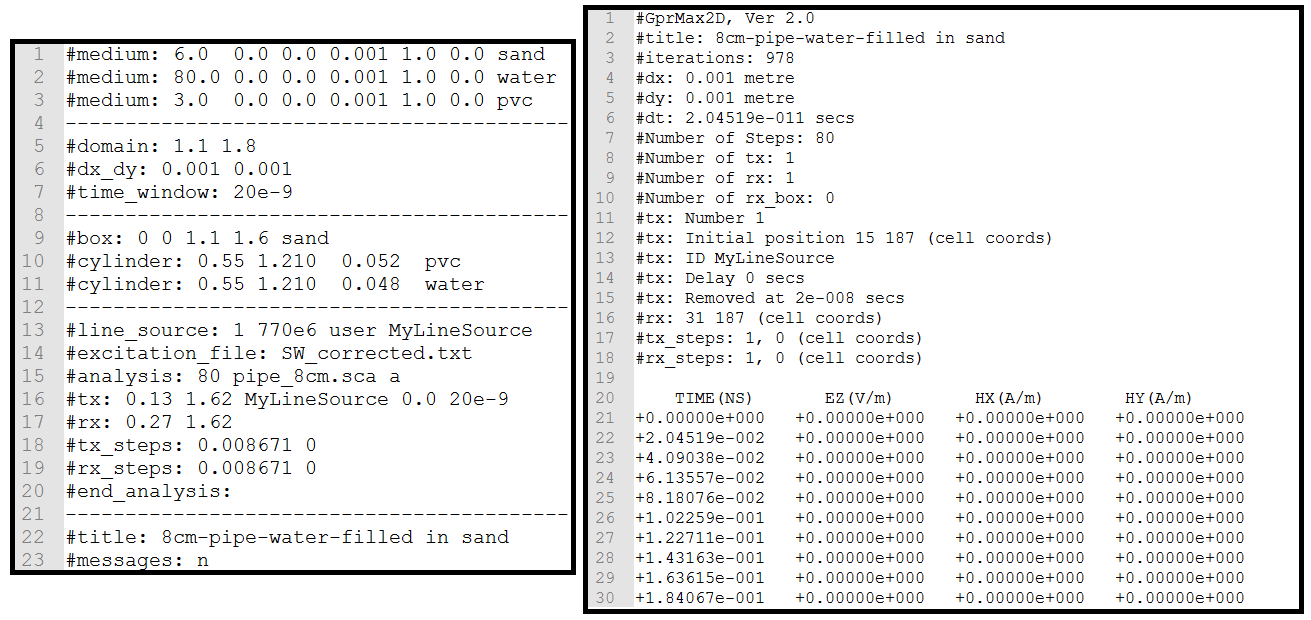
\includegraphics[width=1\linewidth]{gprmax_image.png}
	\caption{gprMax sample input and ASCII output \cite{gprmax}}
\end{figure}
	
\end{block}

%----------------------------------------------------------------------------------------

\end{column} % End of the first column

\begin{column}{\sepwid}\end{column} % Empty spacer column

\begin{column}{\twocolwid} % Begin a column which is two columns wide (column 2)

\begin{columns}[t,totalwidth=\twocolwid] % Split up the two columns wide column

\begin{column}{\onecolwid}\vspace{-.6in} % The first column within column 2 (column 2.1)

%----------------------------------------------------------------------------------------
%	MATERIALS
%----------------------------------------------------------------------------------------

\begin{block}{\textsc{\texttt{Inversion Algorithm}}}

\begin{figure}
	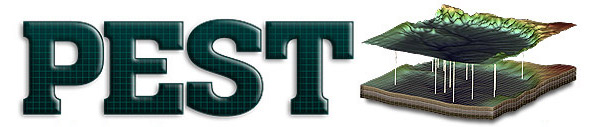
\includegraphics[width=0.8\linewidth]{PEST_flat.jpg}
	\vspace{1cm}
	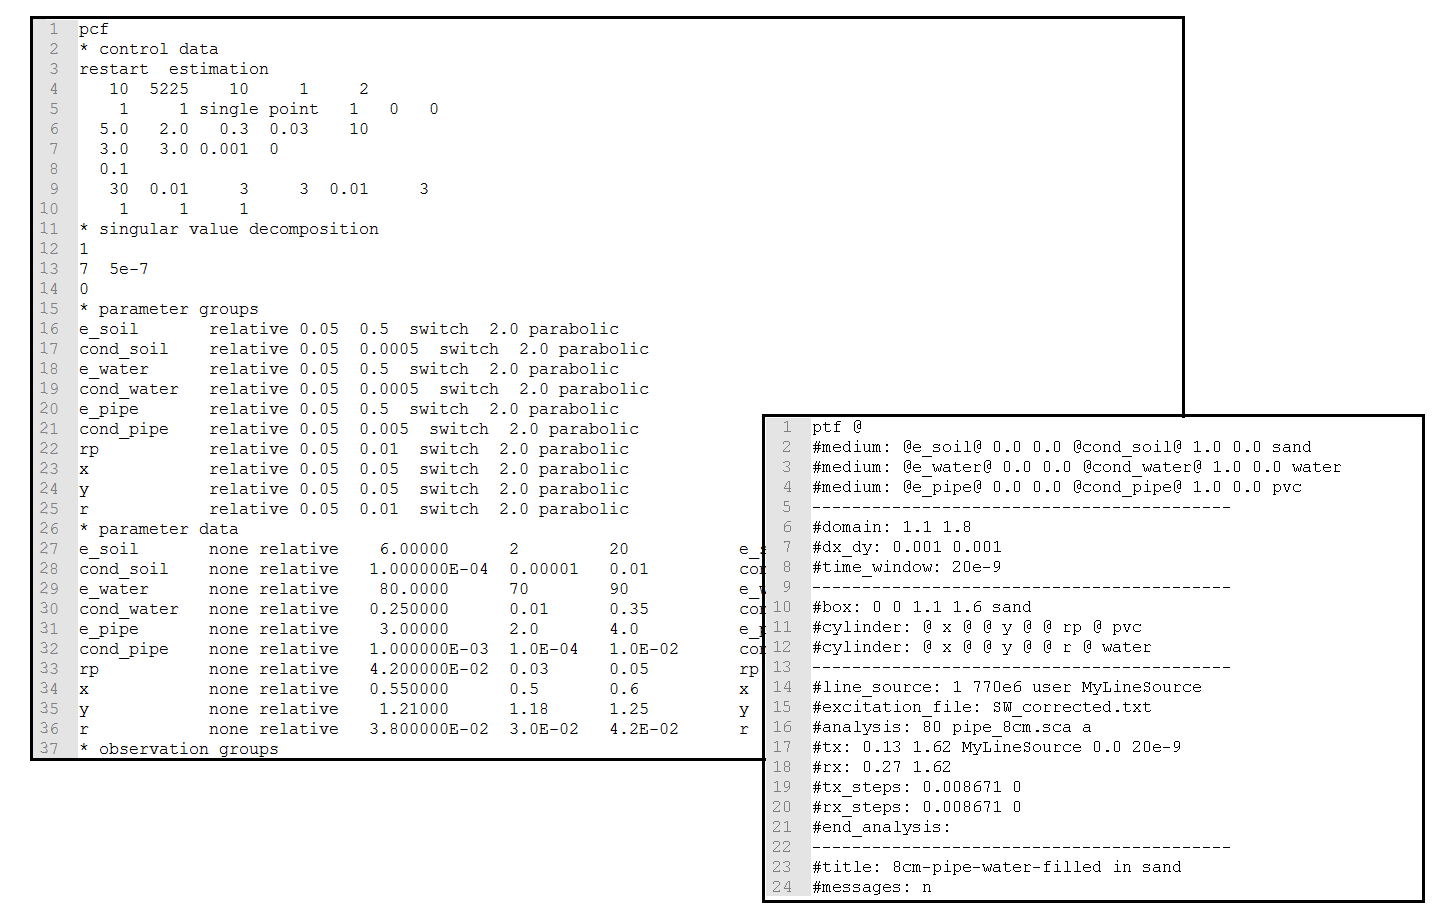
\includegraphics[width=1.05\linewidth]{pest_image.png}
	\caption{PEST sample control and template files~\cite{pest}}
\end{figure}

\end{block}

%----------------------------------------------------------------------------------------

\end{column} % End of column 2.1

\begin{column}{\onecolwid}\vspace{-.6in} % The second column within column 2 (column 2.2)

%----------------------------------------------------------------------------------------
%	METHODS
%----------------------------------------------------------------------------------------

\begin{block}{\textsc{\texttt{ Source Wavelet Estimator}}}
	
Apply \textbf{Sparse Blind Deconvolution} (SBD) to estimate the transmitted waveform. Data are a convolution product of the wavelet and the reflectivity series (impulse response).

%\vspace*{1.5cm}
	\begin{figure}
		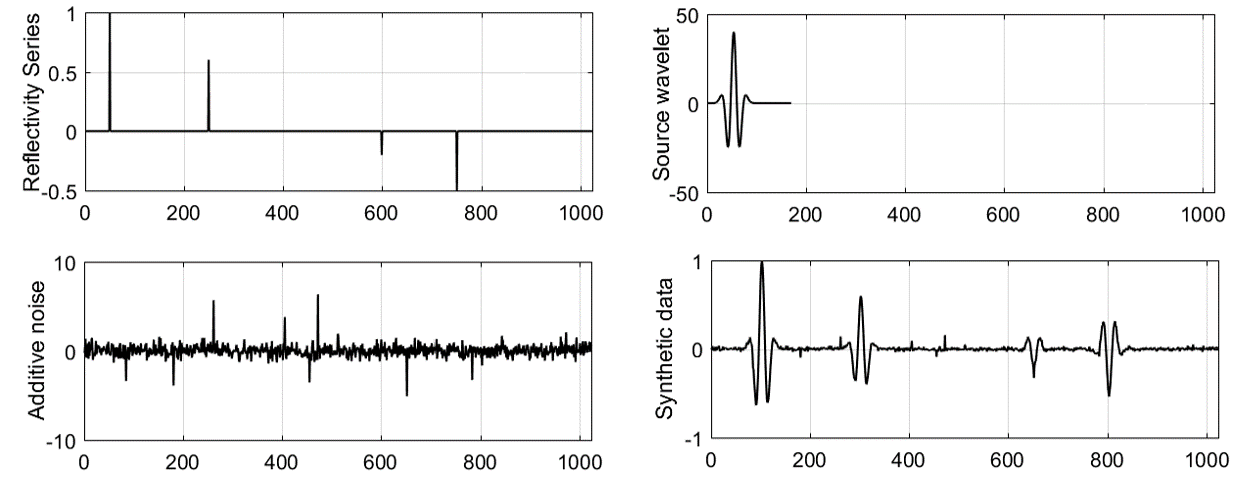
\includegraphics[width=1\linewidth]{synthtic_model_SBD.png}
		\vspace{-3mm}
		\line(1,0){900}
		\vspace{1cm}
		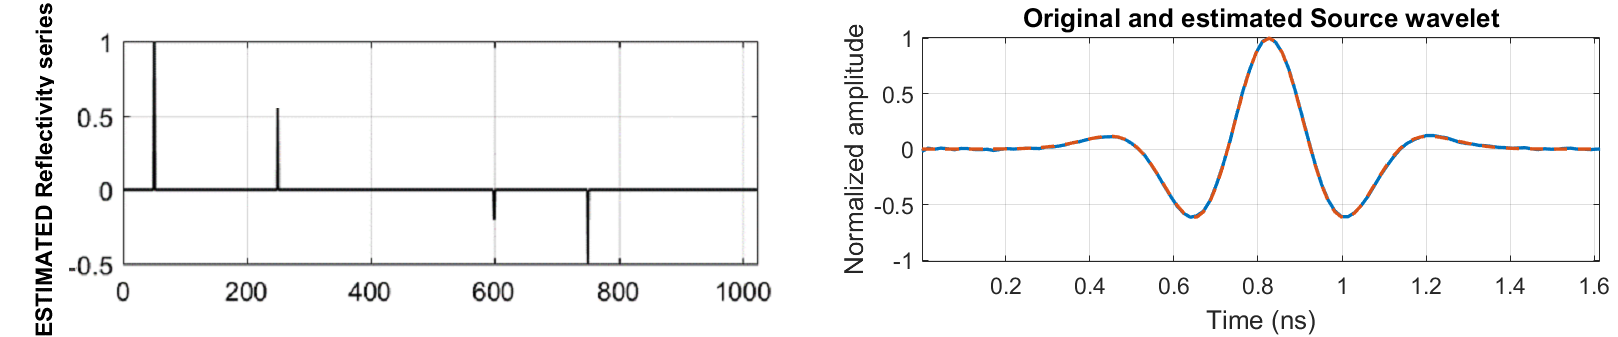
\includegraphics[width=0.98\linewidth]{SBD_synthetic_refl.png}
		\caption{Sparsity based source wavelet estimation (arrivals from the near-field are not used), synthetic case \cite{jazayeri2017sparse}.
		Top: Process of generating synthetic data; Botton: SBD results}
	\end{figure}
	
\end{block}

%----------------------------------------------------------------------------------------

\end{column} % End of column 2.2

\end{columns} % End of the split of column 2 - any content after this will now take up 2 columns width

%----------------------------------------------------------------------------------------
%	IMPORTANT RESULT
%----------------------------------------------------------------------------------------
\vspace{-1cm}
\begin{alertblock}{Key Factors}

FWI is an \textit{iterative process}, in which a good \textbf{starting model} can be improved. It requires traditional data analysis methods to generate a starting model. Similarly, a good estimate of the \textbf{source wavelet} is required.

\end{alertblock} 

%----------------------------------------------------------------------------------------

\begin{columns}[t,totalwidth=\twocolwid] % Split up the two columns wide column again

\begin{column}{\onecolwid} % The first column within column 2 (column 2.1)

%----------------------------------------------------------------------------------------
%	MATHEMATICAL SECTION
%----------------------------------------------------------------------------------------

\begin{block}{\textsc{\texttt{Ray-Based Analyzer}}}

Use ray-based analysis to estimate the initial parameters. For example, we use travel times of the peak amplitudes of the diffraction hyperbola with \textbf{least-squares} approaches to estimate model parameters.  

\begin{figure}
	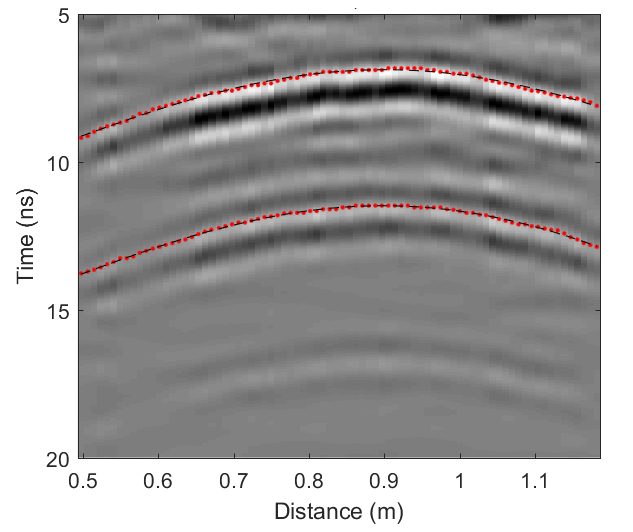
\includegraphics[width=0.7\linewidth]{ray-based.png}
	\caption{Ray-based hyperbola fitting on GPR data over a pipe \cite{jazayeri2017}}
\end{figure}

\end{block}

%----------------------------------------------------------------------------------------

\end{column} % End of column 2.1

\begin{column}{\onecolwid} % The second column within column 2 (column 2.2)

%----------------------------------------------------------------------------------------
%	RESULTS
%----------------------------------------------------------------------------------------
\vspace{-2cm}
\begin{block}{}%{\textsc{\texttt{Ray-based analyzer}}}
\begin{figure}
	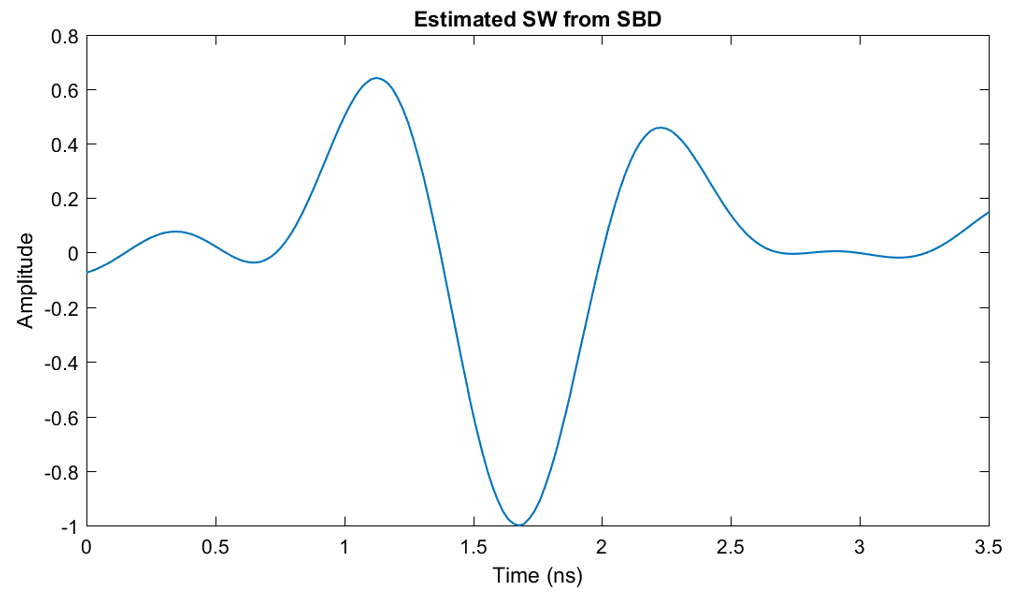
\includegraphics[width=0.4\linewidth]{SBD_pipe_sw.png}
	
	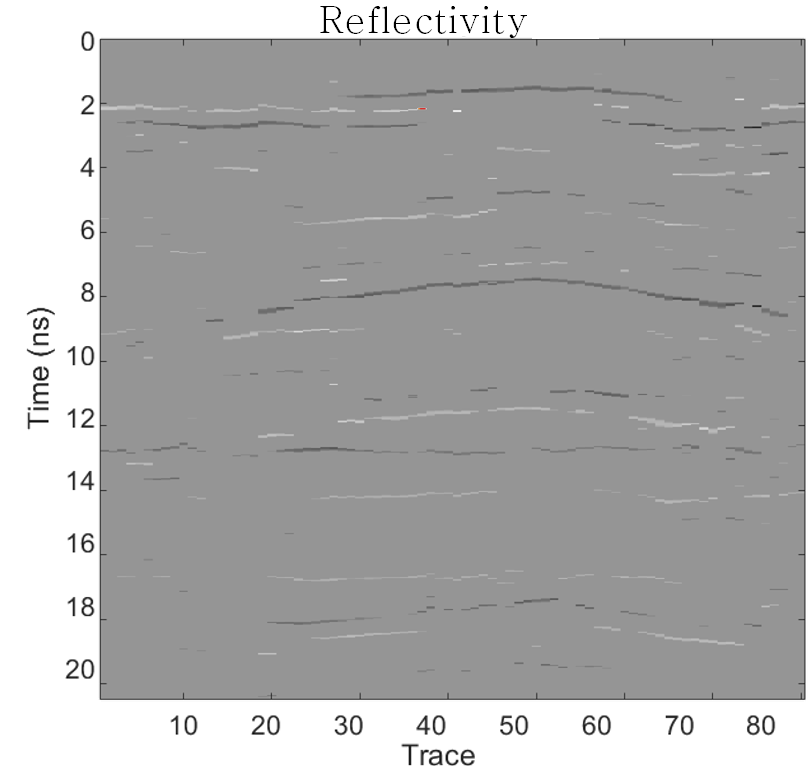
\includegraphics[width=0.65\linewidth]{SBD_pipe_refl.png}
	\caption{\textrm{SBD derived source wavelet and reflectivity series for the real pipe~\cite{jazayeri2017sparse}}}
\end{figure}
\end{block}


%----------------------------------------------------------------------------------------

\end{column} % End of column 2.2

\end{columns} % End of the split of column 2

\end{column} % End of the second column

\begin{column}{\sepwid}\end{column} % Empty spacer column

\begin{column}{\onecolwid} % The third column

\begin{block}{\textsc{\texttt{3D to 2D Converter}}}
	
	Simulate 2D line-source generated waveforms that would be equivalent to those observed in the 3D data, by convolving data in the time domain with $\sqrt{t}$ where $t$ is travel time.
	
\end{block}

\vspace{3cm}

\begin{block}{Example}
	
	\begin{figure}
		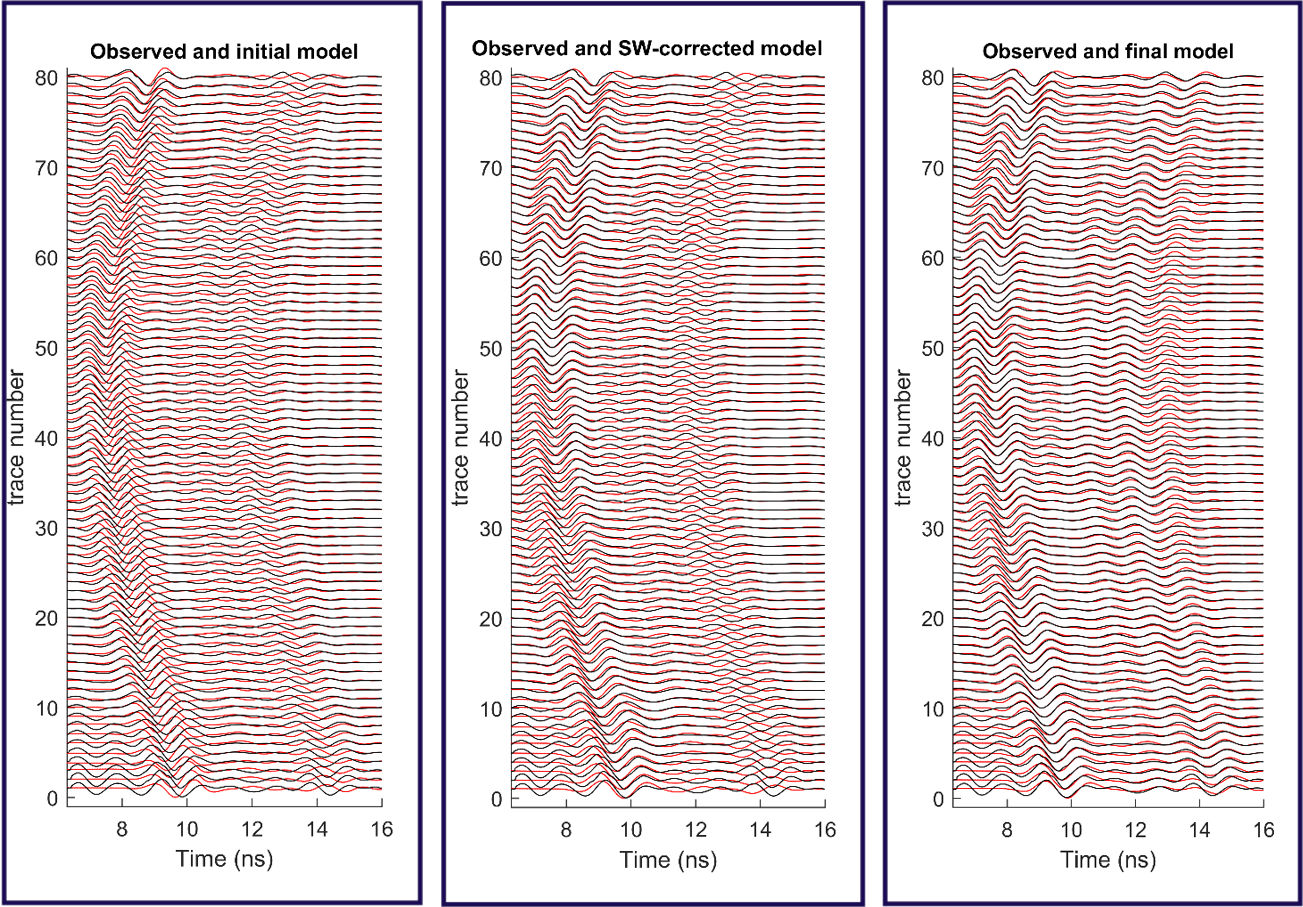
\includegraphics[width=1\linewidth]{FWI_pipes_frames.png}
		\caption{Collected and synthetic pipe data fit after ray-based, SW correction and FWI \cite{jazayeri2017}}
	\end{figure}
	
\end{block}

%----------------------------------------------------------------------------------------
%	ACKNOWLEDGEMENTS
%----------------------------------------------------------------------------------------
\vspace{1.5cm}

\setbeamercolor{block title}{fg=ngreen,bg=white} % Change the block title color

\begin{block}{Acknowledgements}
	
	\small{\rmfamily{We would like to thank Drs. J. Doherty, A. Giannopoulos and C. Warren for making their codes open-source and Mr. A. Ebrahimi for his helpful discussions on SBD.}} \\
	
\end{block}

\vspace{1.5cm}

\begin{block}{References}

\nocite{*} % Insert publications even if they are not cited in the poster
\small{\bibliographystyle{unsrt}
\bibliography{references}\vspace{0.25in}}

\end{block}



%----------------------------------------------------------------------------------------
%	CONTACT INFORMATION
%----------------------------------------------------------------------------------------

\setbeamercolor{block alerted title}{fg=white,bg=jblue!70} % Change the alert block title colors
\setbeamercolor{block alerted body}{fg=black,bg=jblue!5} % Change the alert block body colors


%----------------------------------------------------------------------------------------

\end{column} % End of the third column

\end{columns} % End of all the columns in the poster

\end{frame} % End of the enclosing frame

\end{document}
